\documentclass[10pt]{beamer}
\usetheme[
%%% options passed to the outer theme
%    hidetitle,           % hide the (short) title in the sidebar
%    hideauthor,          % hide the (short) author in the sidebar
%    hideinstitute,       % hide the (short) institute in the bottom of the sidebar
%    shownavsym,          % show the navigation symbols
%    width=2cm,           % width of the sidebar (default is 2 cm)
hideothersubsections,% hide all subsections but the subsections in the current section
%    hideallsubsections,  % hide all subsections
    left               % right of left position of sidebar (default is right)
%%% options passed to the color theme 
%    lightheaderbg,       % use a light header background
  ]{AAUsidebar}

% If you want to change the colors of the various elements in the theme, edit and uncomment the following lines
% Change the bar and sidebar colors:
%\setbeamercolor{AAUsidebar}{fg=red!20,bg=red}
%\setbeamercolor{sidebar}{bg=red!20}
% Change the color of the structural elements:
%\setbeamercolor{structure}{fg=red}
% Change the frame title text color:
%\setbeamercolor{frametitle}{fg=blue}
% Change the normal text color background:
%\setbeamercolor{normal text}{bg=gray!10}
% ... and you can of course change a lot more - see the beamer user manual.

\usepackage{pifont}
\usepackage[utf8]{inputenc}
\usepackage[english]{babel}
\usepackage[T1]{fontenc}
% Or whatever. Note that the encoding and the font should match. If T1
% does not look nice, try deleting the line with the fontenc.
\usepackage{helvet}
\usepackage{wasysym}
\usepackage[export]{adjustbox}
% colored hyperlinks
\newcommand{\chref}[2]{%
  \href{#1}{{\usebeamercolor[bg]{AAUsidebar}#2}}%
}

\title[]% optional, use only with long paper titles
{Development of a Simple Near-Ground Path Loss Model Verified by Measurements\\}

\subtitle{SEMCON 2016}  % could also be a conference name



\author[] % optional, use only with lots of authors
{
Kemal Kapetanovic, Mads Gotthardsen and Thomas Jørgensen
  %Group 16gr651
  %\href{mailto:jkn@es.aau.dk}{{\tt jkn@es.aau.dk}}
}

\date{December 22, 2016}
% - Give the names in the same order as they appear in the paper.
% - Use the \inst{?} command only if the authors have different
%   affiliation. See the beamer manual for an example

\institute[
%  {\includegraphics[scale=0.2]{aau_segl}}\\ %insert a company, department or university logo
  16gr651\\
  1'th Semester WCS
] % optional - is placed in the bottom of the sidebar on every slide
{% is placed on the title page
  16gr651\\
  1'th Semester WCS
  
  %there must be an empty line above this line - otherwise some unwanted space is added between the university and the country (I do not know why;( )
}


% specify a logo on the titlepage (you can specify additional logos an include them in 
% institute command below
%\pgfdeclareimage[width=5 cm]{titlepagelogo}{AAUgraphics/frontpageCropped.png} % placed on the title page
%\pgfdeclareimage[height=1.5cm]{titlepagelogo}{AAUgraphics/aau_logo_newOLD}
%\pgfdeclareimage[height=1.5cm]{titlepagelogo2}{graphics/aau_logo_new} % placed on the title page
\titlegraphic{% is placed on the bottom of the title page
 			 %\pgfuseimage{titlepagelogo}
             
\includegraphics[width = 0.2\textwidth]{AAUgraphics/aau_logo_newOLD.pdf}
%  \hspace{1cm}\pgfuseimage{titlepagelogo2}
}

\usepackage{tikz}
\usepackage[framemethod=tikz]{mdframed}
\usepackage[americanresistors,americaninductors,americancurrents, americanvoltages]{circuitikz}

\newmdenv[tikzsetting={draw=black,fill=white,fill opacity=0.7, line width=4pt},backgroundcolor=none,leftmargin=0,rightmargin=0,innertopmargin=0pt,skipbelow=\baselineskip,%
skipabove=\baselineskip]{TitleBox}


\definecolor{blockcolor}{RGB}{112,168,218}

\tikzstyle{blockbig} = [draw, fill=blockcolor, rectangle, 
    minimum height=3em, minimum width=6em]
\tikzstyle{block} = [draw, fill=blockcolor, rectangle, 
    minimum height=2em, minimum width=2em]
    
\tikzstyle{blockbigclear} = [draw, fill=white, rectangle, 
    minimum height=3em, minimum width=6em]
\tikzstyle{blockclear} = [draw, fill=white, rectangle, 
    minimum height=2em, minimum width=2em]
    
\tikzstyle{sum} = [draw, fill=blockcolor, circle, node distance=1.5cm, minimum size=0.6cm]
\tikzstyle{sumclear} = [draw, fill=white, circle, node distance=1.5cm, minimum size=0.6cm]
\tikzstyle{input} = [coordinate]
\tikzstyle{output} = [coordinate]
\tikzstyle{pinstyle} = [pin edge={to-,thin,black}]

\definecolor{thomasred}{RGB}{247,73,15} %217
\definecolor{thomasblue}{RGB}{0,114,189}
\definecolor{thomasyellow}{RGB}{237,179,32}
\definecolor{thomaspurple}{RGB}{126,47,142}
\definecolor{thomasgreen}{RGB}{119,172,48}
\usepackage{colortbl}

\begin{document}
\setbeamertemplate{caption}{\raggedright\insertcaption\par}
% the titlepage
 {\aauwavesbg%  
%\usebackgroundtemplate{\includegraphics[width=\paperwidth]{frontpage.pdf}}
\begin{frame}[plain,noframenumbering] % the plain option removes the sidebar and header from the title page
\maketitle
%    \begin{figure}[!htbp]
%    \centering
%    \includegraphics[width=0.8\textwidth]{frontpageCropped.png}
%    \end{figure}
\end{frame}}

%%%%%%%%%%%%%%%%
\section{Introduction}
\begin{frame}{Introduction}
\begin{minipage}{0.3\textwidth}
\begin{itemize}
\item Relevance
\item Background
\item Focus
\end{itemize}
\end{minipage}
\begin{minipage}{0.69\textwidth}
\begin{figure}[!htbp]
 \centering
  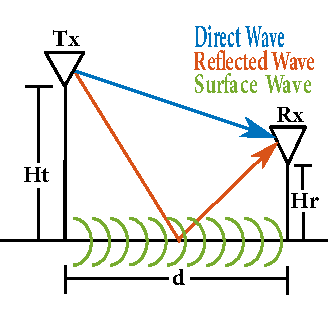
\includegraphics[width = \columnwidth]{figures/poster_cropped_1.pdf}
  \end{figure}
\end{minipage}
\end{frame}
 
%
\section{PL models}
\begin{frame}{PL models}
\begin{minipage}{.45\textwidth}
\raggedright\textcolor{thomasblue}{\textbf{Friss free space PL (FSPL)}:}
\begin{itemize}
\item Only direct wave
\item High heights
\end{itemize} 
\vspace{1em}
\raggedright\textcolor{thomasgreen}{\textbf{Norton surface wave PL (NSPL)}:}
\begin{itemize}
\item Only surface wave
\item Low heights
\item Dependent on surface constants
\end{itemize}
\end{minipage}%
\hspace{.12\textwidth}
\begin{minipage}{.41\textwidth}
\raggedright\textcolor{thomasred}{\textbf{Approximated two-ray}}\\
\raggedright\textcolor{thomasred}{\textbf{ground-reflection PL (ATRPL)}:}
\begin{itemize}
\item Direct and reflected wave
\item Medium heights
\end{itemize}

\raggedright\textcolor{thomaspurple}{\textbf{Ground wave PL (GWPL)}:}
\begin{itemize}
\item All waves
\item All heights
\item Dependent on surface constants
\end{itemize} 
\end{minipage}%
\end{frame}



\section{Measurements}
\begin{frame}{Measurements}
\begin{figure}[!htbp]
	\centering
	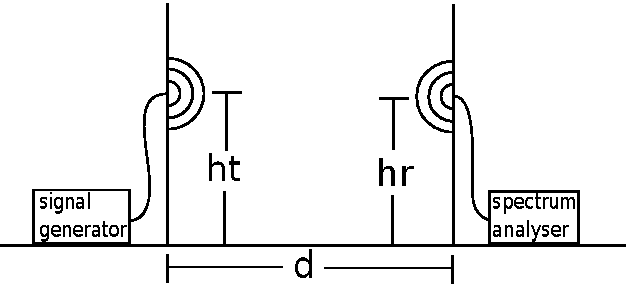
\includegraphics[width = \columnwidth]{figures/setup.pdf}
\end{figure}

\begin{itemize}
\item 1 Frequency (858 MHz)
\item 2 Antenna sets (monopole and patch)
\item 2 Polarization (horizontal and vertical)
\item 2 Location (outdoor and indoor)
\item 4 Rx/Tx heights (from 0.04 to 2.02 m)
\item 6 Distances (from 1 to 30 m)
\end{itemize}
\end{frame}

\definecolor{grey}{RGB}{230,230,230}
\section{Influence of parameters}
\begin{frame}{Influence of parameters}
\begin{table}[!htbp]
\footnotesize
\centering
\textcolor{black}{
\begin{tabular}{|c|c|c|c|}
\hline \rowcolor{black}
\textcolor{white}{Distance}    & \textcolor{white}{1 m} & \textcolor{white}{2 m}& \textcolor{white}{4 m}\\\hline\rowcolor{grey}
PL & (34.7$\pm 1.6$) dB & (41.4$\pm 1.4$) dB & (49.0$\pm 1.7$) dB  \\\hline
\multicolumn{4}{c}{}\\\hline\rowcolor{black}
\textcolor{white}{Distance}	&\textcolor{white}{8 m}& \textcolor{white}{15 m}& \textcolor{white}{30 m}\\\hline\rowcolor{grey}
PL &	(57.3$\pm 2.1$) dB & (66.1$\pm 2.5$) dB & (72.3$\pm 2.3$) dB \\\hline
\end{tabular}}
\end{table}
\begin{table}[H]
\centering
\resizebox{\linewidth}{!}{
\textcolor{black}{
\begin{tabular}{|c|c|c|c|c|}
\hline\rowcolor{black}
\textcolor{white}{Tx \textbackslash Rx} &\textcolor{white}{ 0.04 m} & \textcolor{white}{0.14 m} &\textcolor{white}{ 0.36 m} &\textcolor{white}{ 2.02 m} \\\hline\rowcolor{grey}
\cellcolor{black}\textcolor{white}{0.04 m} & (63.7$\pm 5.2$) dB & (60.7$\pm 5.1$) dB & (55.4$\pm 4.7$) dB & (52.4$\pm 3.8$) dB\\\hline
\cellcolor{black}\textcolor{white}{0.14 m} & (60.7$\pm 5.1$) dB & (58.1$\pm 5.2$) dB & (53.4$\pm 4.5$) dB & (50.2$\pm 3.2$) dB\\\hline\rowcolor{grey}
\cellcolor{black}\textcolor{white}{0.36 m} & (55.4$\pm 4.7$) dB & (53.4$\pm 4.5$) dB & (49.0$\pm 2.9$) dB & (47.6$\pm 4.8$) dB\\\hline
\cellcolor{black}\textcolor{white}{2.02 m} & (52.4$\pm 3.8$) dB & (50.2$\pm 3.2$) dB & (47.6$\pm 4.8$) dB & (44.4$\pm 3.1$) dB\\\hline
\end{tabular}}}
\end{table}


\begin{table}[H]
\centering
\resizebox{\linewidth}{!}{
\begin{tabular}{|c|c|c|c|c|c|}\hline \rowcolor{black}
\multicolumn{2}{|c}{\textcolor{white}{Environment}} & \multicolumn{2}{|c}{\textcolor{white}{Antenna type}} & \multicolumn{2}{|c|}{\textcolor{white}{Polarization}}\\\hline\rowcolor{grey}
Gym & (52.4$\pm 1.8$) dB & Monopole & (55.6$\pm 2.0$) dB &Vertical & (51.8$\pm 1.9$) dB \\\hline
Parking lot & (54.6$\pm 2.2$) dB & Patch & (51.4$\pm 2.0$) dB &Horizontal & (55.1$\pm 2.1$) dB \\\hline
\end{tabular}}
\end{table}
\end{frame}

\section{Model fit}
\begin{frame}{Model fit}

\end{frame}

\section{Proposed model}
\begin{frame}{Proposed model}

\end{frame}

\section{The z parameter}
\begin{frame}{The z parameter}

\end{frame}


%%%%%%%%%%%%%%%%
{\aauwavesbg
\begin{frame}[plain,noframenumbering]
  \finalpage{Questions}
\end{frame}}
%%%%%%%%%%%%%%%%

\end{document}

